\section{Graph-Based Robotic World Models For Dynamic Environments}\label{sec:dyn_world_model_representations}
The evolution of world model representation in robotics has undergone a significant paradigm shift, transitioning from rigid, static geometric maps to adaptive, spatio-temporal structure capable of handling and reasoning about dynamic environments \cite{bavle_slam_2023} \cite{rosinol_kimera_2021}.
In this section, we first review factor graphs as geometric probabilistic backbones (Section \ref{sec:dyn_world_model_representations_factor_graphs}), scene graphs as semantic abstractions (Section \ref{sec:dyn_world_model_representations_scene_graphs}) in dynamic environments, and finally discuss how dynamics themselves are represented (Section \ref{sec:dynamics_representations}).

\subsection{Representational Foundations}
\subsubsection{Factor Graphs as Dynamic Geometric World Models}\label{sec:dyn_world_model_representations_factor_graphs}
To mitigate the impact of outliers and non-stationarity in dynamic environments, factor graph-based systems employ a range of probabilistic robustness mechanisms.
A common approach is the use of \textbf{robust cost functions}, such as the Huber loss, which reduce the influence of large residuals during nonlinear least-squares optimization while preserving sensitivity to small, consistent measurement errors\cite{song_rts-slam_2025}. 
This allows the optimizer to tolerate transient violations of the static-world assumption, caused for instance by moving objects or short-time occlusions, without destabilizing the global solution.
Complementary to robust kernels, \textbf{dynamic information reweighting strategies} explicitly modulate the contribution of individual factors based on their consistency with the current state estimate \cite{lingzhu_xiang_robust_2015}. 
Techniques such as Dynamic Covariance Scaling (DCS) or switchable constraints introduce latent scaling variables that adaptively downweight measurements whose residuals are incompatible with the inferred global structure, providing a principled outlier rejection.
Beyond measurement-level robustness, more expressive models introduce \textbf{latent mobility or existence variables} associated with landmarks or objects, which explicitly encode the likelihood that an entity linked to that variable is static, movable, or currently in motion \cite{lingzhu_xiang_robust_2015}.
By scaling the corresponding factor covariances or relaxing constraints when mobility is inferred, these approaches prevent dynamic or semi-static entities from corrupting the static map while still allowing them to be represented within the same probabilistic framework.
Together, these mechanisms transform factor graphs from purely static geometric estimators into uncertainty-aware models capable of reasoning under dynamic, partially observable conditions.
% To mitigate the impact of outliers in dynamic environments, such as moving objects or spurious loop closures, explicit probabilistic techniques are employed:
% \begin{itemize}
%     \item Robust Kernels: The Huber cost function is frequently applied to downweight large residual, providing a robust optimization back-end that prevents the solution from degrading due to extreme outliers while balancing sensitivity to small residuals\cite{song_rts-slam_2025}.
%     \item Dynamic Scaling: mechanisms like Dynamic Covariance Scaling (DCS) or switchable constraints regularize Mahalanobis errors by dynamically scaling the information matrices of individual edges based on their consistency with the global state \cite{lingzhu_xiang_robust_2015}.
%     \item Latent Mobility Variables: advanced models introduce scalar latent parameters ($\mathit{w}_j$) for each landmark, effectively scaling the covariance to loosen constraints for moving/movable entities, pushing their distribution toward uniformity and neutralizing their influence on the static map \cite{lingzhu_xiang_robust_2015}.
% \end{itemize}
Recently, many works \cite{bescos_dynaslam_2021} \cite{giberna_dynemo-slam_2025} \cite{brink_using_2016} \cite{deeb_model-based_2019} have integrated semantic priors transforming the factor graph from a purely geometric map into a context-aware reasoning engine, facilitating the coupling with other graphical models such as scene graphs.  

Traditional SLAM systems are optimized for a static world treating moving objects and agents as outliers to be rejected \cite{bescos_dynaslam_2018} \cite{bavle_s-graphs_2025}. 
Modern dynamic SLAM instead incorporates these dynamic entities into the graph, moving towards a coupled SLAMMOT approach that is examined in detail in Section \ref{sec:dynamics_representations_agents}.
%Modern dynamic SLAM instead incorporates these dynamic entities into the graph to simultaneously estimate camera trajectory and object motion, therefore enhancing the system robustness and the expressiveness of the resulting world model \cite{deeb_model-based_2019} \cite{gou_visual_2024} \cite{henein_dynamic_2020} \cite{morris_dynosam_2025}, moving towards a coupled SLAMMOT approach, combining SLAM and Multi-Object Tracking. 

\subsubsection{Scene Graphs as Structured Abstraction in Dynamic World Models}\label{sec:dyn_world_model_representations_scene_graphs}
\begin{comment}
The conceptual shift from dense, low-level metric maps towards 3D Scene Graphs represents a significant advancement in robotic world modeling. 
This offers an abstract, layered representation that bridges the gap between the raw geometric perception and high-level symbolic reasoning \cite{bavle_slam_2023}.
By decomposing an environment into a graph structure $G=(V,E)$ robots can move beyond flat representations, such as occupancy grids or point clouds, to models that capture the semantic and relational architecture of the world.  

The literature distinguishes between two primary structural paradigms for scene graphs: 
\begin{itemize}
    \item Flat Scene Graphs: these models treat all entities equally at a single level of representation, focusing on object-level nodes and their direct relationships \cite{catalano_3d_2025}. Systems such as ConceptGraphs\cite{gu_conceptgraphs_2023} and SceneGraphFusion\cite{wu_scenegraphfusion_2021} utilize this approach to manage open-vocabulary object recognition and incremental updates in cluttered scenes where clear structural hierarchies may be emergent rather than predefined. 
    \item Hierarchical Scene Graphs: these represent the environment across multiple levels of abstraction, grouping lower level elements into semantically richer containers, e.g. objects within rooms, rooms within buildings\cite{rosinol_3d_2020} \cite{bavle_s-graphs_2025}. This multi-resolution approach is crucial for scalability in large-scale environments, as it allows robots to perform long-term planning and inference over compact abstractions rather than dense data \cite{catalano_3d_2025}.  
\end{itemize}

Hiearchical frameworks like Hydra \cite{hughes_hydra_2022} and S-Graphs\cite{bavle_s-graphs_2025} adopt a bottom-up stack comprising distinct layers specifically for indoor environments:
\begin{enumerate}
    \item Metric-Semantic Mesh, Pointcloud.
    \item Objects and Agents.
    \item Places and Structures.
    \item Rooms and Floors
    \item Building.
\end{enumerate}
Extending these works to outdoor scenes, \cite{greve_collaborative_2024} proposed hierarchical 3D urban scene graph comprising 6 layers: 
\begin{enumerate}
    \item Keyframes \& Point clouds.
    \item Lane Graph.
    \item Vehicles.
    \item Landmarks.
    \item Roads \& Intersections.
    \item Environment.
\end{enumerate}
\end{comment}
Dynamics in scene graphs are typically handled through three complementary mechanisms operating at different temporal and semantic levels. 
\textbf{Spatio‑temporal consistency} is addressed by separating short‑term dynamics from long‑term structure: systems such as Khronos maintain a fast \textit{active window} to absorb immediate changes due to moving humans or objects, while a slower global process detects persistent changes and updates the long‑term scene graph accordingly \cite{schmid_khronos_2024}. 
Beyond short‑term consistency, some approaches explicitly model recurring temporal patterns. 
The Aion framework augments hierarchical scene graphs with \textit{Maps of Dynamics} (MoDs), attaching directional, time‑dependent \textbf{dynamic temporal flow} statistics to navigational nodes in order to capture typical or seasonal human motion patterns, while using \textit{Temporal Ownership Transfer} to preserve these dynamics under loop closures and graph reorganization \cite{catalano_aion_2025}. 
Finally, \textbf{belief and persistence reasoning} is used to cope with partial observability and object permanence. 
Belief Scene Graphs introduce probabilistic \textit{blind nodes} to represent entities expected to exist but not currently observed, inferred from learned commonsense co‑occurrence patterns \cite{saucedo_estimating_2025}, while interaction‑driven systems such as DovSG perform localized graph updates during human–object interactions, reflecting state changes without requiring a full scene rescan \cite{yan_dynamic_2025}.
Together, these approaches show an evolution of scene graphs from static semantic hierarchies toward persistent spatio-temporal memories that represent not only current scene state but also change, recurrence, and expected future activity.
% Dynamics in scene graphs are handled through various maintenance and prediction mechanisms: 
% \begin{itemize}
%     \item Spatio-Temporal Consistency: to manage changes like moving furniture and humans, systems like Khronos \cite{schmid_khronos_2024} factorize the problam into a fast \textit{active window} for short-term dynamics and a slower global process for long-term change detection.
%     \item Temporal Flow Dynamics: the Aion framework \cite{catalano_aion_2025} integrates Maps of Dynamics (MoDs) into hierarchical scene graphs, attaching directional flow statistics to navigational nodes to predict typical/seasonal human motion patterns over time. It uses Temporal Ownership Transfer to maintain consistency when nodes are repositioned during loop closures.  
%     \item Belief and Persistence: Belief Scene Graphs (BSG) employ probabilistic inference to estimate the existence of "blind nodes", i.e. unseen objects, based on commonsense co-occurance patterns \cite{saucedo_estimating_2025}. Other systems, such as DovSG \cite{yan_dynamic_2025}, perform local graph updates during interaction to reflect real-world state changes, e.g. an object being moved, without the need of a full scene rescan. 
% \end{itemize}

\begin{comment}
Edges in a 3DSG encode the connections within the world model through several relationship types: 
\begin{itemize}
    \item Spatial Relations: These include geometric constraints such as \textit{on}, \textit{in}, \textit{adjacent to} and \textit{support} \cite{catalano_3d_2025} \cite{yan_dynamic_2025}.
    \item Visibility and Proximity: \textit{Co-visibility} edges link objects seen simultaneously, while \textit{close-to} edges often use nearest-neighbourg k-d tree to define spatial proximity \cite{behrens_lost_2025}.
    \item Functional Relations: a newer class of edges representing operational dependencies. OpenFunGraph models these as directed edges between "interactive elements", such as switches and handles, and objects that they influence, e.g. \textit{controls} a light, \textit{opens} a cabinet \cite{zhang_open-vocabulary_2025}.
    \item Affordances: attributes or edges that define possible interactions which can change the entities states, such as \textit{sit on}, \textit{opening}, \textit{pulling}, providing the robot with actionable knowledge \cite{catalano_3d_2025}.
    \item Containment and Affiliation: Inter-layer edges such as \textit{part of}, \textit{located in} or \textit{contains} facilitate hierarchical queries \cite{catalano_3d_2025} \cite{behrens_lost_2025}.
\end{itemize}
This structured abstraction allows robots to move beyond simple obstacle avoidance, static mapping and localization, towards actionable spatial perception, where the world model serves as a persistent, queryable memory for complex multi-step tasks in evolving robot-human shared spaces.
\end{comment}

%\subsection{The Key Bridge}\label{sec:world_model_representation_key_bridge}
\begin{comment}
A scene graph answers "what exists and how it relates". A factor graph answers "where it is, and how certain, consistent with sensors it is".
Many robotics 3DSG systems explicitly include a pose-graph layer as the uncertainty-bearing backbone, and the integration of these two paradigms creates a multi-resolution framework which bridges metric-semantic perception with high-level symbolic reasoning \cite{rosinol_kimera_2021} \cite{bavle_situational_2022}.
In this hybrid paradigm, factor graphs serve as the probabilistic geometric backbone, while scene graphs provide the relational architecture necessary for task-level autonomy in dynamic environments \cite{catalano_3d_2025} \cite{rosinol_3d_2020}.
\end{comment}
%% architecural patterns
%\subsubsection{Architectural Patterns}
\begin{comment}
The literature converges on a small set of recurring architectural patterns for coupling the two paradigms, each representing different trade-off between integration tightness and modularity.
The most prevalent pattern is the \textbf{layered stack with factor graph backbone}: the factor graph simultaneously optimizes the robot's trajectory and the metric-semantic mesh, whose globally and temporally consistent output is then fed to a separate scene graph parser that builds the relational structure on top. 
Hydra \cite{hughes_hydra_2022} and Kimera \cite{rosinol_kimera_2021} support this approach, where a dedicated parsing thread incrementally constructs the scene graph from the optimized metric layer. 
The advantage is modularity, where the scene graph logic can be developed independently of the SLAM back-end, but the disadvantage is a one-directional information flow: the scene graph is informed by the factor graph, but semantic information rarely propagates back to improve localization.

A tighter alternative is the \textbf{single unified optimizable graph}, in which scene graph entities are incorporated directly as variables and factors within the same factor graph that optimizes robot poses. 
S-Graphs \cite{bavle_s-graphs_2025} and its visual counterpart vS-Graphs \cite{tourani2026vs} exemplify this pattern, merging SLAM and scene graph into a single multi-layered jointly optimizable factor graph where walls, rooms, and floors appear as semantic variables constrained by geometric factors.
This enables bidirectional information flow: geometric observation constrain semantic entity positions, but semantic structural priors in turn constrain and regularize ego-trajectory estimation, demonstrably reducing drift compared to purely geometric approaches.
DynEMo-SLAM \cite{giberna_dynemo-slam_2025} extend this to dynamic entities, adding factor graph variables for dynamic entities poses that are simultaneously constrained by semantic motion model priors and structural floor-entity relations. 
A third pattern, the \textbf{loosely coupled parallel architecture}, maintains the factor graph and scene graph as separate optimization problems connected only through shared nodes positions, avoiding the computational cost of joint optimization at the expense of weaker consistency guarantees \cite{rosinol_3d_2020}.
\end{comment}

\begin{figure}
    \centering
    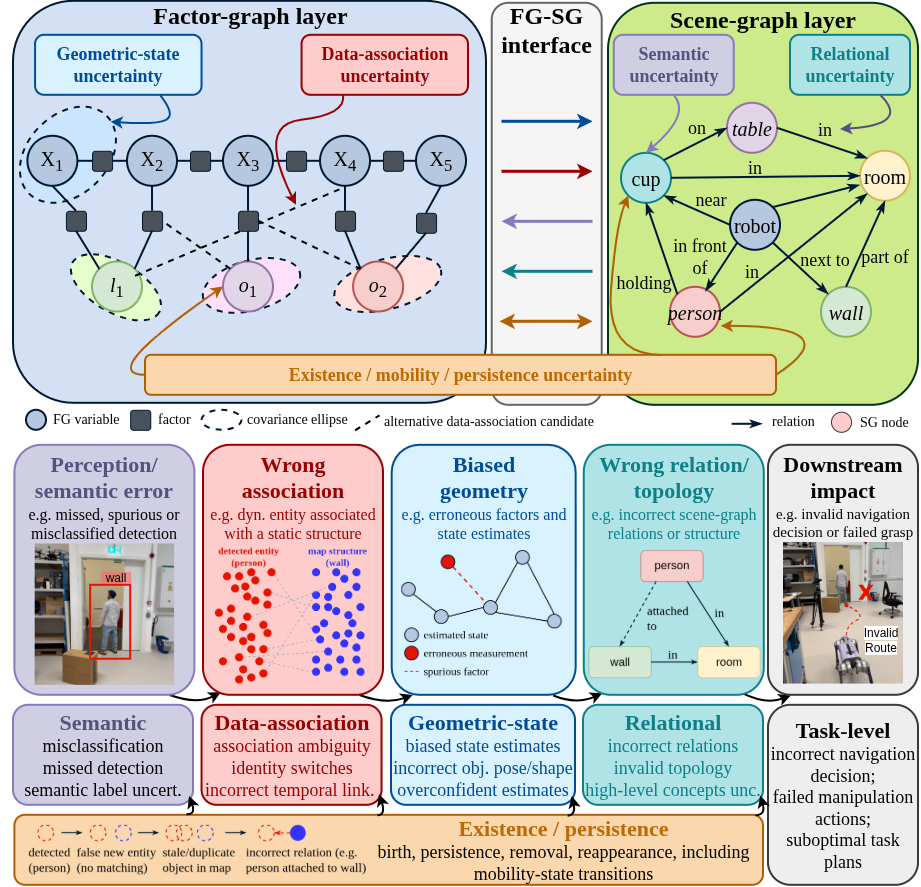
\includegraphics[width=0.99\columnwidth]{Figures/figure_FG_SG_uncertainty_boundary_new_final.png}
    \caption{Uncertainty types and their interface in hybrid factor graph-scene graph world models.}
    \label{fig:FG_SG_uncertainty_boundary}
\end{figure}


%% Uncertainty propagation across the FG-SG boundary
\subsubsection{Uncertainty Types, Propagation, Failure Modes, and Scalability}\label{sec:uncertainty_types}
Uncertainty in graph-based world models does not constitute a single interchangeable quantity, but arises over different latent variables and decisions throughout the representation pipeline.
We distinguish five uncertainty classes that recur across the surveyed approaches: (i) \textit{geometric-state uncertainty}, concerning continuous quantities such as robot poses, landmark positions, object poses, and motion; (ii) \textit{semantic uncertainty}, concerning class labels, attributes, or other learned semantic predictions; (iii) \textit{data-association uncertainty}, concerning which observation corresponds to which existing entity; (iv) \textit{existence uncertainty}, concerning whether an entity is present, persists, disappeared, or should be instantiated; and (v) \textit{relational uncertainty}, concerning the validity of scene-graph edges between entities. 
These uncertainty classes characterize the uncertain quantities or hypotheses represented by the world model and should be distinguished from the sources of uncertainty entering the inference process. 
For geometric estimation in particular, sensor and odometry noise appear as measurement uncertainty on observation factors, while imperfect motion or structural assumptions introduce model uncertainty through prior factors. 
Both contribute to the posterior uncertainty of geometric state variables.
These uncertainty classes differ both in their mathematical representation and in how they propagate through the world model.
Consequently, a system can provide a principled probabilistic treatment for one class while treating others deterministically or through heuristic confidence measures.

\begin{table*}[t]
\centering
\caption{Uncertainty classes in graph-based dynamic world models.}
\label{tab:uncertainty_classes}
\renewcommand{\arraystretch}{1.15}
\setlength{\tabcolsep}{4pt}
\scriptsize
\begin{tabularx}{\textwidth}{
    >{\raggedright\arraybackslash}p{0.07\textwidth}
    >{\raggedright\arraybackslash}p{0.16\textwidth}
    >{\raggedright\arraybackslash}p{0.23\textwidth}
    >{\raggedright\arraybackslash}p{0.23\textwidth}
    >{\raggedright\arraybackslash}X}
\hline
\textbf{Uncertainty class} &
\textbf{Uncertain quantity} &
\textbf{Typical representation / treatment} &
\textbf{Representative mechanisms} &
\textbf{Main cross-layer issue} \\
\hline

Geometric state &
Robot/object pose, landmark position, velocity motion &
Measurement/odometry factor noise models; motion-prior/model covariance; posterior state covariance or information &
Probabilistic factor-graph estimation and smoothing; marginal covariance estimation; adaptive or learned factor covariance &
Propagation from geometric states to scene-graph entities and relations \\

Semantic &
Class labels, attributes, semantic observations &
Learned class probabilities or confidence measures; uncertainty-weighted semantic factors &
Semantic perception; learned semantic factor uncertainty &
Calibration and transfer of perception uncertainty into probabilistic estimation \\

Data association &
Observation-to-entity correspondence &
Discrete hypotheses, association probabilities, latent or switchable variables &
JPDA, MHT, weighted or switchable constraints &
Incorrect associations alter graph structure and cannot be represented by state covariance alone \\

Existence &
Entity presence, persistence, birth, and removal &
Bernoulli existence probability; Random Finite Set intensities and mixtures &
Bernoulli, PHD, and PMBM filtering; persistence and decay models &
Coupling probabilistic birth/death estimates to scene-graph node lifecycle \\

Relational &
Validity of scene-graph edges or predicates &
Learned probabilities or heuristic confidence measures; often deterministic &
Spatial, semantic, and functional relation inference &
Propagation of endpoint-state and semantic uncertainty into relation confidence \\

\hline
\end{tabularx}
\end{table*}


These uncertainty classes, summarized in Table \ref{tab:uncertainty_classes}, interact but cannot generally be propagated using the same mechanism. 
Geometric-state uncertainty is continuous and naturally represented within factor-graph inference, whereas data association and existence involve discrete hypotheses or latent variables. 
Semantic uncertainty originates primarily from learned perception and may influence factor weights or association decisions, while relational uncertainty concerns higher-level graph structure.
Errors can therefore propagate across classes: uncertain semantics may induce an incorrect association, an incorrect association may bias geometric estimation, uncertain existence may trigger premature node deletion, and uncertain endpoint states may invalidate a scene-graph relation. 
A central limitation of current hybrid FG-SG systems is that these cross-class dependencies are rarely represented within a single probabilistic model.

Across the surveyed systems, these five classes exhibit markedly different degrees of explicit probabilistic treatment. Geometric-state uncertainty is the most systematically represented: factor-graph-based approaches routinely associate measurement and prior factors with covariance or information models and propagate their effect through state estimation.
Semantic uncertainty is less consistently preserved: learned perception front-ends often provide class probabilities or confidence scores, but these are frequently converted into deterministic labels before entering the world model or used only to modulate selected factor weights.
Data association uncertainty is similarly heterogeneous: although probabilistic multi-hypothesis formulations such as JPDA and MHT provide explicit distributions over correspondences, many practical systems commit to deterministic geometric, appearance, or learned-similarity matches. 
Existence uncertainty is generally handled through persistence scores, decay rules, or geometric verification, while explicit Bernoulli/RFS-based existence probabilities remain uncommon in integrated FG-SG systems. 
Relational uncertainty is the least developed class: scene-graph predicates are commonly instantiated deterministically or accompanied by learned confidence scores, with little explicit propagation of uncertainty from their endpoint states.
The uncertainty profiles reported in Table \ref{tab:taxonomy_overview} reflect this imbalance, with probabilistic treatment concentrated primarily in geometric estimation and substantially weaker probabilistic support toward semantic and relational layers.

The consequences of neglecting these uncertainty classes are also different. 
Mischaracterized measurement or motion-model uncertainty changes the weighting of geometric factors and can produce overconfident or biased state estimates.
Incorrectly calibrated semantic confidence may alter factor weighting or association decisions.
Data-association errors are more severe structurally. Once an observation is assigned to the wrong entity, a small conditional pose covariance does not represent the uncertainty of that assignment. Poor existence modeling produces either stale entities or premature deletion, while overconfident relational inference can propagate uncertain geometric or semantic states into incorrect high-level graph edges consumed by planning and reasoning.
These failure modes therefore cannot be diagnosed or mitigated through geometric covariance alone.

Geometric-state uncertainty is the most mature of these classes within factor-graph formulations. Measurement factors, including sensor observations and odometry constraints, encode measurement uncertainty through noise models, covariance matrices, or information matrices.
Motion-prior factors similarly encode uncertainty associated with the assumed evolution model.
These uncertainties are fused through probabilistic inference, and posterior marginal state covariances can be obtained from the resulting joint information matrix, commonly using a local Gaussian approximation around the MAP estimate \cite{dellaert_factor_2017}.
\textcolor{red}{The difficulty arises at the boundary: how does the uncertainty of the pose nodes in a factor graph propagate into the semantic and relational claims made by a scene graph node?
In the layered-stack architecture, this propagation is largely absent, as shown in Figure \ref{fig:FG_SG_uncertainty_boundary}.
Scene graph nodes that are instantiated from a poorly constrained region of the pose graph  carry the same confidence as one from a well constrained area. 
In dynamic settings, where uncertainty is generally higher and crucial for spatio-temporal estimation and prediction, this is a large drawback.
Systems that adopt the unified optimizable graph architecture handle this more naturally: by representing semantic entities as factor graph variables, their states participate in the joint information structure, allowing their posterior uncertainty to reflect the geometric and semantic constraints included in the optimization \cite{bavle_s-graphs_2025}.}
\hl{At the FG-SG interface, it is important to distinguish uncertainty representation from uncertainty propagation. 
The former concerns which uncertainty quantities are explicitly modeled, whereas the latter concerns how their uncertainty affects estimates or beliefs in another representation.
In a layered architecture, geometric-state uncertainty can be propagated forward by transferring state distribution, marginal covariances, or appropriate approximations alongside the optimized geometric states. This does not require semantic feedback to the factor graph.

However, when only point estimates or deterministic labels are transferred, information about uncertainty and correlations may be lost at the interface. Even when marginal covariances are retained, dependencies between entities may be discarded, limiting the subsequent assessment of relational uncertainty. 

In unified optimizable graph architectures, the geometric states of semantic entities participate directly in the joint estimation problem, as in S-Graphs} \cite{bavle_s-graphs_2025}. \hl{This allows their posterior uncertainty to reflect the dependencies encoded by the included factors.
Nevertheless, joint MAP estimation does not imply that posterior covariances are explicitly recovered, nor that uncertainty over semantic labels, entity existence, or scene-graph relations is represented probabilistically.}
\hl{For example, consider the relative position between two scene-graph entities, $\mathbf{d_{ij}} = \mathbf{p_i} - \mathbf{p_j}$. Its covariance is given by:}
\begin{equation}
    \Sigma_{d_{ij}} = \Sigma_{ii} + \Sigma_{jj} - \Sigma_{ij} - \Sigma_{ji}
\end{equation}
\hl{where $\Sigma_{ii}$ and $\Sigma_{jj}$ denote the marginal position covariances, and $\Sigma_{ij}$ and $\Sigma_{ji}$ their cross-covariances. Transferring only individual state estimates or marginal covariances may therefore be insufficient to correctly characterize the uncertainty of a spatial relation. This illustrates that the preservation of statistical dependencies across representation layers is distinct from the direction of information flow.}
\hl{Existing systems demonstrate different aspects of uncertainty handling rather than a complete cross-representation propagation mechanism. For instance, Kimera} \cite{rosinol_kimera_2021} \hl{ and Hydra }\cite{hughes_hydra_2022} \hl{perform Bayesian fusion of semantic observation at the voxel level, but this is distinct from propagating geometric posterior uncertainty into scene-graph relations. Similarly, the joint estimation of geometric states associated with semantic entities in S-Graphs does not by itself provide probabilistic beliefs over all semantic and relational attributes.}
Recent work by Millan-Romera et al. \cite{millanromera2026generationuncertaintyawarehighlevelspatial} demonstrates that incorporating learned uncertainty estimates for semantic factors, rather than fixed information matrices, further improves SLAM accuracy, particularly in edge cases where semantic concepts are the only cues preserving geometric consistency.

A poorly-constrained dynamic entity node produces an unreliable trajectory estimate that, if allowed to influence loop-closure candidates, can corrupt the static map, too\cite{giberna_dynemo-slam_2025}.
%Khronos \cite{schmid_khronos_2024} addresses this through explicit 4D metric uncertainty on object fragments, distinguishing reliable observations from transient ones before any graph level update is triggered. 
Khronos \cite{schmid_khronos_2024} mitigates this by \textcolor{red}{attaching explicit 4D metric uncertainty to its object fragments before they are committed to the global graph, rather than treating every instantiated node as equally confident.} \hl{aggregating locally consistent observations into object fragments, jointly optimizing fragment positions and robot poses using robust geometric constraints, and performing geometric verification before reconciling fragments into persistent objects. 
These mechanisms improve the robustness of the resulting representation, but do not constitute explicit propagation of posterior geometric uncertainty into higher-level semantic relations.} 
The broader challenge, i.e., consistent propagation of geometric and temporal uncertainty into semantic relations, (e.g., how certain is the \textit{on} edge between an object and a table, given the covariance on both their pose nodes?) remains largely open and represents one of the key research gaps identified in Section \ref{sec:challenges_future_works}.

A related failure mode in dynamic environments is the corruption of higher-level scene graph abstractions by incorrect dynamic entity handling. 
If a moving person is incorrectly associated with a static wall node during a period of high dynamics, the resulting factor introduces a misleading constraint into the joint optimization that can displace the wall node and corrupt the room topology built on top. 
This cross-layer error propagation is difficult to detect and correct a posteriori, motivating the use of explicit confidence gating to prevent semantically inconsistent observations from entering the graph \cite{zhang_outlier_2023}.
Viewed end-to-end, these errors form a propagation chain rather than isolated module failures. 
A missed or incorrect detection can create a missing or misclassified entity, an incorrect association can lead to an erroneous factor and bias the estimated state, biased states can in turn affect scene-graph relations or topology. 
Downstream modules then consume this corrupted representation, so an incorrect relation or object state may ultimately produce an invalid navigation decision or manipulation task. 
Robust complete systems therefore require uncertainty and consistency checks across the interfaces between perception, estimation, abstraction and action, rather than only within individual modules.
Importantly, errors are not propagated uniformly across this chain.
Continuous measurement errors may be attenuated through repeated observations, robust factor weighting, and joint optimization, whereas discrete errors such as incorrect identity association, false entity instantiation, or premature deletion can alter the graph structure itself and persist across subsequent updates.
The interfaces between perception, association, estimation, and abstraction therefore act either as error filters or error-amplification points.
Temporal aggregation and robust estimation can suppress noisy observations before they affect the persistent model, while an incorrect committed association can create a structurally valid but semantically wrong factor that subsequently biases geometric states and higher-level relations.

%% computation scalability
The trade-off between representational richness and real-time inference is a challenge for hybrid factor graph-scene graph systems.
As the environment grows, both the factor graph and the scene graph accumulate nodes and edges, and the computational cost of optimization scales with graph density.
Several strategies have been developed to manage this.
\textit{Hierarchical optimization} exploits the layered structure of scene graphs to scope optimization to the relevant subgraph: S-Graphs 2.0 \cite{bavle_s-graphs_2025} runs room-level local optimization continuously and floor-level global optimization only on loop closure, avoiding full re-optimization of the entire graph at each update.
\textit{Marginalization and sparsification} are applied at the factor graph layer to maintain a bounded-size active window, with older variables marginalized into prior factors. 
DynoSAM \cite{morris_dynosam_2025} and its hybrid world-object centric formulation \cite{morris_online_2025} use embedded-frame anchoring (Section \ref{sec:construction_pipeline_backend}) to preserve sparsity as dynamic object maps grow.
\textit{Task-driven graph pruning}, detailed in Section \ref{sec:querying_reasoning_action_action}, reduces the relational superstructure to a minimal actionable subgraph relevant to the current task, as in Clio \cite{maggio_clio_2024} and SayPlan \cite{rana2023sayplangroundinglargelanguage}, preventing the planning complexity from growing with the full map. 
Together these strategies allow hybrid systems like Khronos \cite{schmid_khronos_2024} and DynEMo-SLAM \cite{giberna_dynemo-slam_2025} to achieve real-time performance in complex large indoor environments. However, the scalability of unified optimizable graphs to large-scale, highly dynamic outdoor scenes where both the agent population and the structural complexity are greater, remains an active research direction and will be discussed in more detail in Section \ref{sec:construction_pipeline_backend}.




% The literature converges on a hierarchical layer stack where the factor graph explicitly grounds the scene graph nodes in a shared spatial reference frame. 
% This leads to having at the base \textbf{the Geometric Foundation}, a metric semantic mesh/point cloud which provides spatial grounding \cite{rosinol_3d_2020}. This layer is frequently maintained by factor graph optimizers, which simultaneously optimze the robot's trajectory and the mesh vertices or point cloud during loop closures to maintain global consistency. 
% Next, the \textbf{Object-Agent Layer} follows, categorizing entities into generally-static objects and time-varying agents. In dynamic settings, agents are represented as secondary pose graphs within the factor graph, capturing their trajectories as sequences of time-stamped pose variables \cite{giberna_dynemo-slam_2025}.
% On top, the \textbf{Relational Superstructure} contains topology nodes that are connected to the underlying metric landmarks through inter-layer edges, allowing high-level reasoning such as resolving queries like "which objects are in this rooms" or "which objects is next to this one" while maintaining the geometric precision needed for navigation. 

Figure \ref{fig:unifying_view_SG_FG} summarizes this hybrid architecture, showing how the factor graph backbone and scene graph superstructure connect through shared dynamic modeling and graph-maintenance stages to support downstream querying, reasoning and action.
This unified representation enables actionable spatial perception, where the world model is not merely a passive map but a persistent, query-able substrate for planning, interaction, and scene prediction.

\begin{figure}
    \centering
    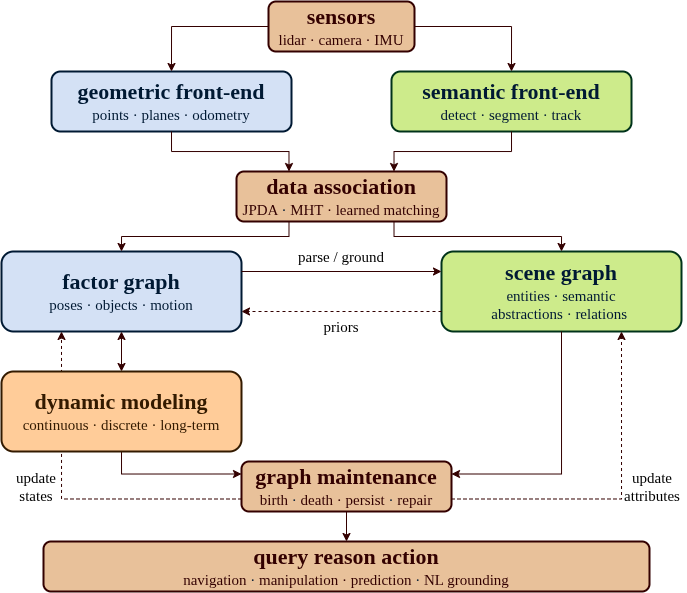
\includegraphics[width=\columnwidth]{Figures/figure_FG_SG_architecture.png}
    \caption{Conceptual architecture of a hybrid probabilistic graph-based dynamic world model.}
    \label{fig:unifying_view_SG_FG}
\end{figure}

\subsection{Representing Dynamics in Graph-Based World Models}\label{sec:dynamics_representations}
The evolution of world model representations for robotics in non-stationary scenarios has progressed from treating environmental change as outlier noise toward a systematic, relational and probabilistic characterization of dynamics across multiple temporal scales \cite{rosinol_3d_2020} \cite{schmid_khronos_2024}.
This section presents the most common characterization of dynamic entities in dynamic world modeling. Specifically, we emphasize the integration of factor graphs and 3DSGs to handle short-term dynamics (Section \ref{sec:dynamics_representations_agents}), semi-static changes (Section \ref{sec:dynamics_representations_objects}), and long-term structural evolution (Section \ref{sec:dynamics_representations_longterm}). 
Figure \ref{fig:dynamics_timescale} depicts the dynamic distinction we adopt \textcolor{red}{, based on the type and temporal scale of expected motion}, highlighting \hl{typical but non-defining temporal ranges and} some relevant works focusing on each of them.

\begin{figure}[!ht]
    \centering
    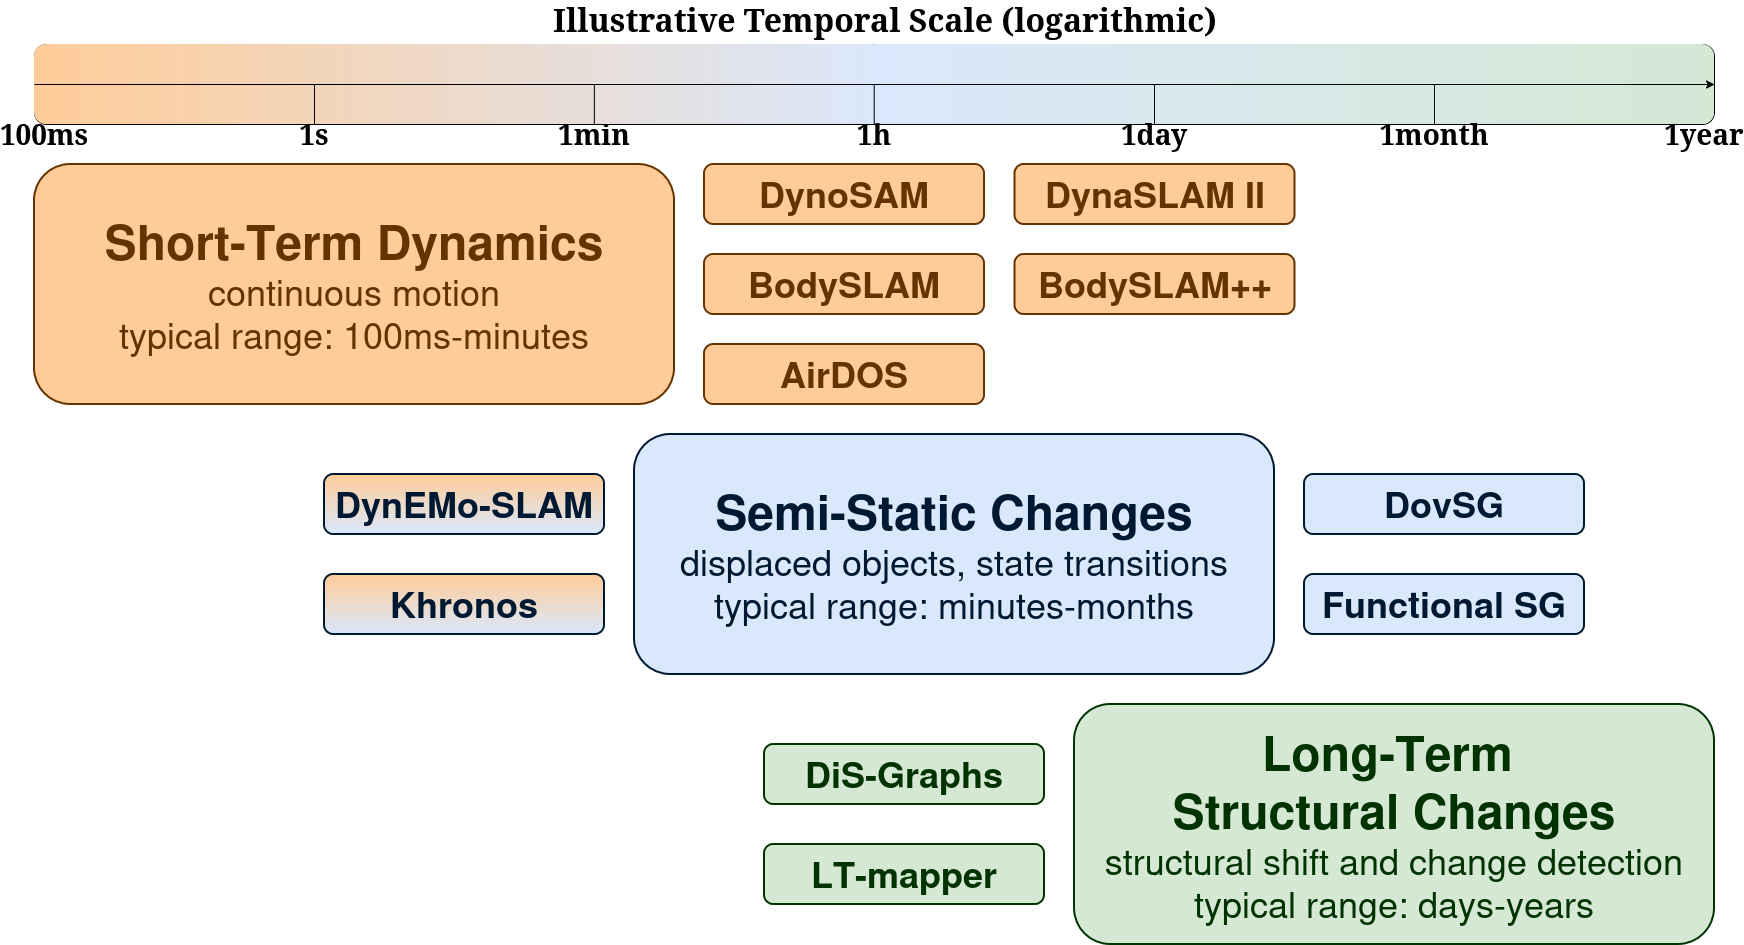
\includegraphics[width=0.9\columnwidth]{Figures/figure_dynamics_timescale_updated.png}
    \caption{Diagram showing the adopted  temporal-horizon taxonomy. \hl{The reported temporal ranges are indicative of typical timescales and do not constitute fixed classification boundaries.} The tiers denote operational change regimes \hl{relative to the robot's observation and wold model update horizons,} rather than mutually exclusive entity classes\textcolor{red}{, t} \hl{. T}he same entity or system may span multiple tiers. Relevant works are reported for each, or group of, type of dynamics.}
    \label{fig:dynamics_timescale}
\end{figure}


\subsubsection{Short-Term Dynamics}\label{sec:dynamics_representations_agents}
In an environment populated by humans and/or moving objects, the world model must resolve the ``motion ambiguity'' where pixel or point displacement is a compound effect of the simultaneous robot's ego motion and the independent motion of other entities \cite{zhang_semantic-integrated_2026}. 

%% Separate static Map vs Dynamic Layer (Loosely coupled SLAMMOT)
Early paradigms typically treated short-term dynamic entities as outliers to be masked or rejected \cite{bescos_dynaslam_2018} to preserve the consistency of a purely static map. 
Contemporary loosely coupled systems often maintain these as separate threads, using the camera pose as a prior for multi object tracking (MOT) but without allowing object measurements to refine the ego-localization\cite{tian_dl-slot_2024} \textcolor{red}{\cite{tian_dl-slot_2024}} \cite{gou_visual_2024}. 
In this way, a uni-directional flow of information is generated, allowing the optimized static map data, output of the SLAM process, to enhance MOT but not the other way around.

%% Fully Coupled Joint optimization frameworks
Modern representations employ a tightly-coupled SLAMMOT approach, where the factor graph back-end jointly optimizes camera poses, static landmarks, and the trajectories of dynamic objects or agents within a unified optimization manifold \cite{zhang_semantic-integrated_2026}.
Systems like DynaSLAM II \cite{bescos_dynaslam_2021}, DynEMo-SLAM \cite{giberna_dynemo-slam_2025}, SMMF-SLAMMOT \cite{zhang_semantic-integrated_2026} support a tightly-coupled approach where robot poses, static landmarks, and dynamic entity trajectories are jointly optimized in a unified factor graph.
This paradigm requires spatio-temporal reprojection factors to introduce cross-terms between camera poses and object motions, ensuring that the estimation of self and the surrounding is mutually beneficial. 
% employ spatio-temporal reprojection factors that couple geometric observations across frames to enforce rigid-body kinematic constraints, effectively improving both self-localization and object tracking accuracy. 
%% Hybrid Efficiency 
To address the computational effort of joint optimization, DynoSAM\cite{morris_dynosam_2025} and Hybrid iSAM2 \cite{morris_online_2025} formulations anchor rigid body motions to ``embedded frames'', preserving graph sparsity as each object map grows while enabling efficient incremental inference by a Bayes Tree. 
% This allows each object map to grow as new fragments become visible while preserving graph sparsity, enabling efficient incremental inference via the Bayes Tree.

%% Coordinate frame representation (MOVED to VI-A)
% A critical design choice involves the coordinate frames used for agents states. 
% While object-centric formulations express points in a local body frame to enforce rigidity, recent analysis indicates that world-centric or hybrid representations, which anchor motions to an "embedded frame" established at the first observation, superiorly preserve factor graph sparsity and enhance solver efficiency for incremental optimizers like iSAM2 \cite{morris_importance_2024} \cite{morris_online_2025}.

%% Agent specific states
% Humans are often represented with specific node types containing 3D pose graphs for their trajectories and non-rigid shape models, such as Skinned Multi-Person Linear Model (SMPL) meshes \cite{loper_smpl_2015}, ensuring the world model accounts for both articulated motion and volumetric presence \cite{rosinol_kimera_2021} \cite{schmid_khronos_2024}.
% TODO go deeper in SMPL, bodyslam and bodyslam++ and other human models
Humans represent a particularly important and challenging sub-class of short-term dynamics, often referred to as \textit{dynamic agents}: they are simultaneously the most common source of dynamics in real-world environments and the most structurally complex entity to model. This stems from the fact that humans fall into the challenging \textit{articulated} and \textit{goal-driven} categories along the typology and behavioral intent axes, respectively.
Systems like Kimera \cite{rosinol_kimera_2021} and Khronos \cite{schmid_khronos_2024} represent humans with dedicated node types combining 3D pose graph trajectories with non-rigid models, ensuring the world models account for both articulated motion and volumetric presence. 
BodySLAM \cite{henning_bodyslam_2022} and its successor BodySLAM++ \cite{henning_bodyslam_2023} push this further, pioneering the joint optimization of camera trajectory and dense human body shape and pose within a single factor graph, where each human observation is a parametric body model linked to the camera pose graph via reprojection factors. 
BodySLAM++ \cite{henning_bodyslam_2023} extends this to multiple simultaneous human instances, integrating inertial factors in a real-time fashion, improving robustness to occlusion in crowded scenes. 
In both cases, the structured prior provided by the body model regularizes an otherwise underconstrained problem, the same role played by rigid-body kinematic priors for object-class short-term dynamics, like for instance in \cite{qiu2022airdos} accounting for dynamic articulated objects.

%% human body models
The choice of the body model determines the degrees of freedom exposed to the optimizer and the computational costs of inference. 
Parametric models dominate in SLAM-integrated systems: SMPL \cite{loper_smpl_2015} represents the body as a compact, differentiable parameter vector via linear blend skinning, making it naturally compatible with factor graph optimization \cite{henning_bodyslam_2022}\cite{henning_bodyslam_2023}.
SMPL-X \cite{SMPL-X:2019} extends this to hands and face, while STAR \cite{STAR:2020} reduces blend skinning artifacts at extreme poses. 
For monocular initialization without depth sensors,  learned estimators such as VIBE \cite{kocabas2019vibe}, FrankMocap \cite{rong2021frankmocap}\cite{joo2020eft} and PromptHMR \cite{wang2025prompthmr} provide  body-model parameters. 
At the opposite end,  METRO \cite{lin2021end-to-end} directly predicts mesh vertices, while  InstantAvatar \cite{jiang2022instantavatar}  learns a subject-specific neural representation. These approaches replace the compact fixed-dimensional parameterization of SMPL-family models with higher-dimensional representations that are less directly suited to integration as factor-graph state variables. 
The prevailing trade-off is therefore between the structured compactness of SMPL-family models and the expressiveness of learned representations, summarized in Table~\ref{tab:body_models}.

\begin{table*}[t]
\centering
\caption{Comparison of human body representations and inference methods relevant to robotic world modeling.}
\label{tab:body_models}
\resizebox{\textwidth}{!}{
\begin{tabular}{llllllll}
\toprule
\textbf{Model} & \textbf{Input} & \textcolor{yellow}{\textbf{Method Type}} & \textbf{Hardware} & \textbf{Training} & \textbf{Output} & \textbf{Body Parts} & \textbf{Use Case} \\
\midrule

SMPL \cite{loper_smpl_2015}
& Shape/pose params
& Parametric body model
& CPU/GPU
& Offline (scan-based)
& Parametric mesh
& Body only
& SLAM, MOT, animation \\

SMPL-X \cite{SMPL-X:2019}
& Shape/pose/expr.\ params
& Parametric expressive body model
& GPU
& Offline (scan-based)
& Parametric mesh
& Body + hands + face
& Expressive HRI, animation \\

STAR \cite{STAR:2020}
& Shape/pose params
& Parametric body model
& CPU/GPU
& Offline (scan-based)
& Parametric mesh
& Body only
& SLAM, extreme pose recovery \\

Anny \cite{bregier2025humanmeshmodelinganny}
& Phenotype params
& Parametric phenotype-conditioned body model
& CPU/GPU
& None (scan-free)
& Parametric mesh
& Body + hands + face
& Diverse pop.\ modeling, HMR \\

VIBE \cite{kocabas2019vibe}
& Monocular video
& Temporal SMPL regressor
& GPU
& Offline (video data)
& SMPL params/frame
& Body only
& Video-based pose init. \\

FrankMocap \cite{rong2021frankmocap} \cite{joo2020eft}
& RGB image
& Whole body regressor + integration
& GPU
& Offline (images)
& SMPL-X params
& Body + hands
& Real-time monocular HMR \\

METRO \cite{lin2021end-to-end}
& RGB image
& Direct mesh regressor
& GPU (high-end)
& Offline (images)
& Raw mesh vertices
& Body + hands
& Accurate shape recovery \\

PromptHMR \cite{wang2025prompthmr} &
RGB image + spatial/semantic prompts &
Prompt-conditioned mesh regressor &
GPU &
Offline &
SMPL-X parameters &
Body + hands + face &
Promptable multi-person HMR / interaction \\

InstantAvatar \cite{jiang2022instantavatar}
& Monocular video
& Subject-specific neural avatar
& GPU (high-end)
& Per-subject online
& Neural field + mesh
& Full body
& Avatar reconstruction \\

\bottomrule
\end{tabular}
}
\end{table*}

% e.g. moving humans, moving objects... 
% Joint SLAM+tracking: objects nodes have state over time.
% Key question: separate static map vs dynamic layer, or fully coupled?

\subsubsection{Semi-Static Changes}\label{sec:dynamics_representations_objects}
Semi-static dynamics involve objects that are stationary during observation but relocated over time, ending up displaced in future observations \cite{brink_using_2016} \cite{giberna_dynemo-slam_2025}.
This requires the model to distinguish between ``moving'' and ``movable'' states. 
Additionally, it is needed to learn what kinds of changes a specific entity can undergo and how to handle object disappearance. 

%% State variables and changes and Affordances
Nodes in modern 3DSGs are annotated with dynamic attributes such as \textit{open/closed} or \textit{on/off} \cite{olivastri_multi-modal_2024}. 
These properties, often inferred via Vision-Language Models \cite{shao_large_2025}, define \textit{functional scene graphs} \cite{rotondi_fungraph_2025} \cite{zhang_open-vocabulary_2025} where interactive elements like handles are linked to the objects they trigger, ending up to change their states. 

%% Object Permanence vs Forgetting
The key question of permanence is handled via hierarchy and containment edges (for instance an object in a drawer) \cite{behrens_lost_2025} \cite{yan_dynamic_2025}.
Systems like Lost \& Found \cite{behrens_lost_2025} maintain object permanence by updating these relations online. 
If a human hides an item in a drawer, the \textit{contains} edge ensures the robot \textit{remembers} the location despite total occlusion. 

%% Inactive Nodes vs delation
Decisions to prune the graph are often governed by probabilistic decay rates \cite{gomez_object-based_2020} or explicit geometric verification \cite{schmid_khronos_2024}.
In DPG-SLAM \cite{walcott-bryant_dynamic_2012}, sectors of a node are turned off if they intersect with evidence of removal. 
A node is marked inactive if a threshold of sectors is off, but it is only deleted if it no longer provides useful topological information, thereby managing complexity without losing historical data. 
% e.g. moved objects, changed states
% add state variable (open/closed) and persistence logic.
% Key Question: object permanence vs forgetting: when do nodes get deleted vs marked inactive.

\subsubsection{Long-Term Structural Changes} \label{sec:dynamics_representations_longterm}
Lifelong autonomy necessitates a world model that can align multiple sessions and detect structural shifts in the environment \cite{deeb_model-based_2019} \cite{catalano_3d_2025}, precluding the assumption of staticity in entities or parts of the map which would otherwise be considered unmovable in shorter or single-session campaigns.

%% structural change detection
At geometric level, structural change detection compares observations from different sessions to classify map regions as stable, changed or newly appeared. 
DPG-SLAM \cite{walcott-bryant_dynamic_2012} addresses this by continuously comparing current sensor data against submaps from previous sessions.
Regions where contradictions occur are marked as changed, and associated nodes are pruned.
LT-mapper \cite{kim2022lt} extends this to large-scale outdoor LiDAR SLAM through anchor-node-based inter-session loop factors that align drifted session pose graphs into a shared coordinate frame, applying then set-difference operations to identify positive and negative changes at keyframe level.
% Khronos \cite{schmid_khronos_2024} handles this through its spatio-temporal factorization. 
% The asynchronous global process continuously checks the current metric-semantic mesh against the accumulated map, triggering node deactivation when ray-tracing evidence confirms structural removal.

%% multi-session aligment  and graph updates
Merging observations from multiple sessions into a globally consistent factor graph requires solving both the inter-session pose offset and the data association between observation of potentially changed structures.
The standard mechanism is the introduction of inter-session loop closure factors, i.e.,  constraints between nodes from different sessions that share stable landmarks \cite{kim2022lt}.
Memory management is critical to keep this tractable. As shown in \cite{labbe2014online}, a hierarchical short-term/working/long-term memory structure can bound the number of loop closure candidates, enabling multi-session operation under computational constraints. 

%% structural priors
A complementary approach to multi-session alignment uses prior structural knowledge, typically in form of Building Information Models (BIM) or architectural plans, to anchor the factor graph to a known coordinate frame and constrain the estimation of structural elements. 
BIM-SLAM \cite{vega_torres_bim-slam_2023} models both the robot's SLAM graph and the architectural plan as a hierarchical factor graph, then detects inter-session loop closure between them. 
DiS-Graphs \cite{shaheer_tightly_2025} extends this to jointly estimate deviations between the planned and the built environments, incorporating BIM-derived structural priors as soft constraints in the factor graph to remain accurate even when the real building deviates from its original plans.
The key insight in both works lies in the hierarchical scene graph structure, e.g., walls, rooms, floors, which provides a natural alignment target that is more robust to partial scene change than point-level descriptors.
The graph update policy in these systems therefore distinguishes between permanent structural entities, even in cases of deviations or changes, which are retained and used for inter-session alignment, and semi-static or movable entities.
